\documentclass[10pt,twocolumn,letterpaper]{article}

\usepackage{cvpr}              % camera-ready style (author names shown). Use [review] to anonymise.
\usepackage{times}
\usepackage{epsfig}
\usepackage{graphicx}
\usepackage{amsmath}
\usepackage{amssymb}
\usepackage{booktabs}
\usepackage{multirow}
\usepackage{listings}

\usepackage[pagebackref,breaklinks,colorlinks,bookmarks=false]{hyperref}

\def\cvprPaperID{****}
\def\confName{CVPR}
\def\confYear{2022}

\newcommand{\ap}{AP$_{50}$}

\lstset{
  language=Python, basicstyle=\ttfamily\tiny, breaklines=true, breakatwhitespace=false,
  numbers=left, numberstyle=\tiny, numbersep=3pt, columns=fullflexible, keepspaces=true,
  showstringspaces=false, xleftmargin=8pt
}

\hypersetup{pdftitle={Visual Object Search in Drone Images},pdfauthor={Ashish Pratap Singh}}
\begin{document}

%%%%%%%%% TITLE
\title{Visual Object Search in Drone Images}

\author{Ashish Pratap Singh \quad 261010070\\
Indian Institute of Technology Kanpur\\
\texttt{ashishps26@iitk.ac.in}
}

\maketitle

%%%%%%%%% ABSTRACT
\begin{abstract}
Finding every instance of a user-specified object in a high-resolution drone image is difficult: objects cover only a few dozen pixels, scale and appearance vary, and a closed-set detector cannot anticipate new object types. We study \emph{query-by-example search}: given a box around an object in a support image, return all instances of that object in a target drone image, with no training. Our pipeline combines frozen DINOv2 patch features computed on tiles of the target image, a rotation-aware query encoding in which the support window is rotated and re-embedded, template matching over a multi-scale feature pyramid, and a coarse-to-fine step that re-matches the top candidates in a local window at twice the resolution. We evaluate on 117 one-shot episodes built from VisDrone-DET, with queries taken from different images. Coarse-to-fine refinement is the most useful component: on top of a fixed pyramid it raises the mean per-episode \ap{} from 10.6 to 13.6 (paired bootstrap 95\% CI of the difference $[+1.6,+4.4]$) and Recall@100 from 29.2 to 31.7. Rotation-aware encoding adds 4.1 points of Recall@100 but no measurable AP gain, and a pyramid whose scales are derived from the query size did not help (it was slightly worse). A tiled OWL-ViT image-guided baseline reaches 2.4--3.5 \ap{} and is competitive only on large objects. AP rises from 13.5 at IoU~0.5 to 37.8 at IoU~0.1, which shows that box size, inherited from the query, is the main limitation of the current method.
\end{abstract}

%%%%%%%%% BODY TEXT
\section{Introduction}
\label{sec:intro}

Drones are widely used for traffic monitoring, search and rescue, and surveillance. In these settings an operator often wants to ask an ad-hoc question such as ``find all vehicles that look like \emph{this one}'' in a large aerial image. The standard answer is a supervised detector such as YOLO~\cite{redmon2016yolo} trained on a fixed label set (for VisDrone~\cite{zhu2021visdrone}, ten classes). Such a detector cannot find an object type outside its label set without new labelled data and retraining.

\emph{Visual object search} instead takes a single example as the query. The aerial setting makes this hard for four reasons: (i) objects are tiny relative to the image (VisDrone images are about $2000\times1500$ pixels), so downscaling the image erases them; (ii) the same object appears at very different scales depending on altitude; (iii) a top-down camera has no canonical ``up'', so the query may be rotated relative to the target; and (iv) the query comes from a different image, with different lighting and blur.

\noindent\textbf{Problem statement.} \emph{Input:} a target drone image and a query, i.e.\ a bounding box on a support image. \emph{Output:} a ranked list of boxes in the target image that contain the same kind of object, plus the estimated rotation of the match. \emph{Constraints:} no training or fine-tuning for a new object; one example per query; images of up to several thousand pixels.

\noindent\textbf{Approach.} We use frozen DINOv2~\cite{oquab2023dinov2} patch features and treat search as template matching in feature space. The target is tiled so small objects keep their resolution; the query is encoded after rotating the support window by multiples of $90^\circ$; and the best candidates are re-matched in a local window at twice the resolution.

\noindent\textbf{What is and is not new.} The individual ingredients are not new: tiling large aerial images~\cite{akyon2022sahi,xie2022fewer}, DINOv2 patch matching for few-shot tasks~\cite{bou2024fewshot,damm2025anomalydino,espinosa2025notime}, and rotated references~\cite{damm2025anomalydino} all have precedent. We do not claim a new backbone or a first-of-its-kind system; our literature search was limited, so we also cannot rule out closely related prior work. Our contributions are:
\begin{enumerate}
  \item An adaptation of training-free DINOv2 matching to one-shot object search in drone images, with a rotation-aware query encoding that rotates and \emph{re-embeds} the support window (ViT features are not rotation-equivariant), and a coarse-to-fine local refinement step.
  \item An episodic evaluation protocol on VisDrone-DET with cross-image queries, and a component-wise ablation with paired bootstrap confidence intervals.
  \item Evidence on what does and does not help: coarse-to-fine refinement helps AP and recall; rotation helps recall only; a query-size-derived scale pyramid, which we initially expected to be a contribution, did not help.
\end{enumerate}

%------------------------------------------------------------------------
\section{Related Work}
\label{sec:related}

\noindent\textbf{Detection in drone imagery.} Supervised detectors such as YOLO~\cite{redmon2016yolo} are trained on benchmarks like VisDrone~\cite{zhu2021visdrone}, and are closed-set. Large aerial images are usually handled by slicing them into tiles and detecting on each; SAHI~\cite{akyon2022sahi} formalises slicing-aided inference for small objects, and Xie et al.~\cite{xie2022fewer} study efficient detection in large aerial images. We adopt tiling but apply it to feature extraction instead of detection.

\noindent\textbf{Few-shot and image-guided detection.} Few-shot detectors adapt a detector with a few labelled examples~\cite{kang2019fsrw}. OWL-ViT~\cite{minderer2022owlvit} supports image-conditioned (``one-shot'') detection with a pretrained open-vocabulary model; we use it as our baseline. Bou et al.~\cite{bou2024fewshot} study robust features for few-shot detection in satellite imagery, which is the closest work to ours in application; we did not compare against it.

\noindent\textbf{Training-free matching with self-supervised features.} DINOv2~\cite{oquab2023dinov2} patch features support dense correspondence without fine-tuning. AnomalyDINO~\cite{damm2025anomalydino} matches patch features against a few reference images and offers rotation of the references, and Espinosa et al.~\cite{espinosa2025notime} build a training-free reference-based segmentation pipeline on frozen foundation models. Our work follows this training-free line and differs in the target task (box-level search in tiled, high-resolution drone images), the multi-scale kernel matching, and the coarse-to-fine refinement we evaluate.

%------------------------------------------------------------------------
\section{Method}
\label{sec:method}

Figure~\ref{fig:overview} gives an overview. All components use a frozen DINOv2 ViT-B/14 (patch size $P=14$); nothing is learned.

\begin{figure*}[t]
  \centering
  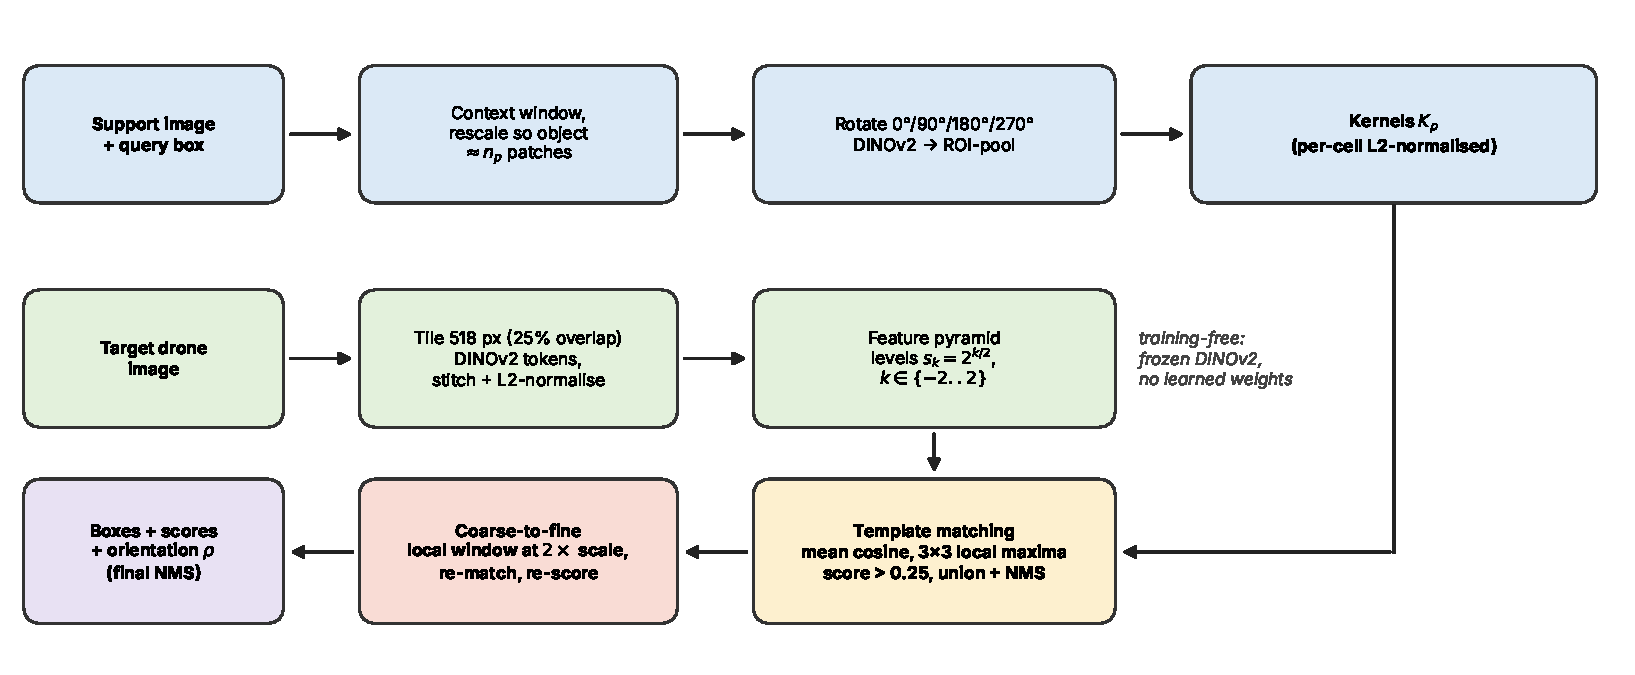
\includegraphics[width=0.92\linewidth]{fig_overview.pdf}
  \caption{Overview of the pipeline. The query branch (top) turns a box on a support image into rotated patch-feature kernels $K_\rho$. The target branch (middle) builds a tiled DINOv2 feature pyramid. Kernels are slid over the pyramid to produce coarse candidates, which are refined in local windows at $2\times$ resolution.}
  \label{fig:overview}
\end{figure*}

\subsection{Dense features for large images}
A target image is resized by a scale $s_k=2^{k/2}$ (level $k$, half-octave steps) and split into $518\times518$ tiles (a $37\times37$ patch grid) with stride 364 pixels. The patch tokens of overlapping tiles are averaged, stitched into one map, and L2-normalised per patch, giving $F_k\in\mathbb{R}^{C\times h_k\times w_k}$. Levels are computed lazily and cached. Levels whose longer side would exceed 4032 pixels are skipped.

\subsection{Rotation-aware query encoding}
Let the query be a box $(x,y,w,h)$ on a support image. We set the rescale factor $r_q = n_p P / \max(w,h)$ so the object spans about $n_p$ patches. A context window around the box (half-size $\max(1.5\max(w,h),\,112/r_q)$) is cropped and rescaled by $r_q$. For each rotation $\rho\in\{0,1,2,3\}$ the \emph{window and a box mask} are rotated by $\rho\cdot90^\circ$ and embedded by DINOv2, and the tokens inside the rotated box are ROI-aligned into a kernel $K_\rho\in\mathbb{R}^{C\times g_h\times g_w}$, which is L2-normalised per cell. Rotating the image before embedding is necessary because ViT features are not rotation-equivariant; it also makes the kernel shape change for odd $\rho$. The best-scoring $\rho$ at a detection is returned as the estimated orientation (we do not evaluate orientation accuracy).

\subsection{Multi-scale template matching}
For level $k$ and rotation $\rho$, the score map is the mean cosine similarity between the kernel and the feature map,
\begin{equation}
S_{k,\rho}(i,j)=\frac{1}{g_hg_w}\sum_{u=1}^{g_h}\sum_{v=1}^{g_w}\big\langle F_k(i+u,j+v),\,K_\rho(u,v)\big\rangle .
\end{equation}
Local maxima ($3\times3$ neighbourhood) with $S>0.25$ become candidates (at most 300 per map). A candidate's box is the (rotated) query box size placed at the kernel centre, divided by the level scale to return to image coordinates; its score is $S$. Candidates from all levels and rotations are merged with NMS (IoU 0.5, at most 300 kept).

\noindent\textbf{Pyramid policies.} \emph{Single scale} uses $k=0$. \emph{Fixed pyramid} uses $k\in\{-2,\dots,2\}$ (scales $0.5$--$2$) for every query. \emph{Query-adaptive pyramid} centres the levels on $k_0=\mathrm{round}(2\log_2 r_q)$, i.e.\ $k\in\{k_0-2,\dots,k_0+2\}$, the level at which an object of the query's size spans $n_p$ patches. We tested the adaptive policy as a possible contribution; Sec.~\ref{sec:results} shows it did not help.

\subsection{Coarse-to-fine refinement}
The top $M=150$ candidates are refined. For a candidate at level $k$ we crop a window of half-size $\max(1.5\,\max(\text{box side}),\,64/s_f)$ around its centre, resize it by $s_f=2s_k$, embed it, and match it with a kernel re-extracted at scale $2r_q$ (same rotation). The match position is searched only within $\pm2$ fine patches of the coarse centre to avoid jumping to a neighbouring instance. The refined score is $\alpha s_{\text{coarse}}+(1-\alpha)s_{\text{fine}}$ with $\alpha=0.5$; unrefined candidates keep $\alpha s_{\text{coarse}}$, so they rank below refined ones. A final NMS gives the output.

%------------------------------------------------------------------------
\section{Experiments}
\label{sec:experiments}

\subsection{Data and protocol}
\noindent\textbf{Dataset.} VisDrone2019-DET~\cite{zhu2021visdrone}: ten object classes plus ``ignored regions''. Annotations list $(x,y,w,h,\text{score},\text{category},\text{truncation},\text{occlusion})$; boxes with score 0 are not counted and detections centred in ignored regions are discarded.

\noindent\textbf{Episodes.} An episode is (target image from the VisDrone \emph{val} split, category $c$, query from a \emph{different} \emph{train} image). The task is to find all instances of $c$ in the target. A category is eligible if the target contains at least three countable instances; at most two categories are sampled per image. Queries are clean instances (score 1, not truncated, not occluded, shorter side $\ge12$ px, longer side $\le300$ px) drawn from every fifth train annotation file. With a fixed seed we obtain \textbf{117 episodes on 60 val images}; all methods see the same episodes.

\noindent\textbf{Metrics.} For each episode we compute AP at IoU 0.5 (all-point interpolation) and Recall@100 (fraction of ground-truth boxes matched by the 100 highest-scoring detections), and report means over episodes; the tables label the AP column \ap{}. This is a per-episode AP and is \emph{not} the class-averaged mAP of standard detection benchmarks, so the numbers are not comparable with published VisDrone results. We also report the runtime per episode (seconds, including feature extraction for the pyramid levels used, excluding image loading) on a single Kaggle GPU. Sizes follow the median longer box side of the category's ground truth in the target: small ($<32$ px), medium (32--64 px), large ($>64$ px).

\subsection{Implementation details}
DINOv2 ViT-B/14 (\texttt{facebook/dinov2-base}, fp16), tile 518 px with stride 364 px, $n_p=4$, $\alpha=0.5$, refinement of the top 150, score threshold 0.25, NMS IoU 0.5. The value $n_p=4$ was chosen after inspecting results on a separate tuning set of val images disjoint from the 60 evaluation images (Appendix~\ref{app:tuning}). We disclose that an earlier $n_p$ sweep on the evaluation episodes themselves suggested the same value; we discarded it and repeated the sweep on held-out images, where the full pipeline actually scored higher at $n_p=3$ than at $n_p=4$, while the non-refined variants preferred $n_p$ of 4 to 5. With only 37 tuning images these differences are small and noisy, so $n_p=4$ should be read as a reasonable choice, not an optimum.

\noindent\textbf{Baseline.} OWL-ViT~\cite{minderer2022owlvit} (\texttt{google/owlvit-base-patch32}) image-guided detection, run on $768\times768$ tiles (stride 576) of the target at $1\times$ and $2\times$ scale, with the query box cropped (15\% margin) from the support image, score threshold 0.05 and NMS. We did not tune the baseline, so its numbers may understate what a tuned OWL-ViT could reach.

\noindent\textbf{Configurations.} All use the same encoder and $n_p=4$:
A single scale; B fixed pyramid; C adaptive pyramid; D adaptive pyramid with 4 rotations; E adaptive pyramid, rotations and refinement; F fixed pyramid with refinement; G fixed pyramid with rotations and refinement. \textbf{F and G were added after we saw the results of A--E} (refinement looked useful, adaptive scales did not), so choosing G as the final method is a post-hoc decision on the same episodes. Treat results involving F and G as exploratory.

\subsection{Results}
\label{sec:results}

\begin{table}[t]
\centering\small
\begin{tabular}{@{}llccc@{}}
\toprule
 & Method & \ap{} & R@100 & s/ep\\
\midrule
A & Single scale & 4.49 & 8.13 & 0.16\\
B & Fixed pyramid & 10.64 & 29.16 & 1.19\\
C & Adaptive pyramid & 8.97 & 28.27 & 1.80\\
D & C + rotation & 8.48 & 30.31 & 1.85\\
E & D + coarse-to-fine & 12.51 & 36.41 & 3.74\\
F & B + coarse-to-fine & \textbf{13.59} & 31.68 & 2.52\\
G & F + rotation (final) & 13.50 & 35.80 & 3.04\\
\midrule
 & OWL-ViT tiled, $1\times$ & 2.36 & 7.28 & 0.63\\
 & OWL-ViT tiled, $2\times$ & 3.54 & 15.29 & 2.58\\
\bottomrule
\end{tabular}
\caption{Mean over 117 episodes (\%, runtime in s/episode). A--E were planned; F and G were added afterwards.}
\label{tab:main}
\end{table}

\begin{figure}[t]
  \centering
  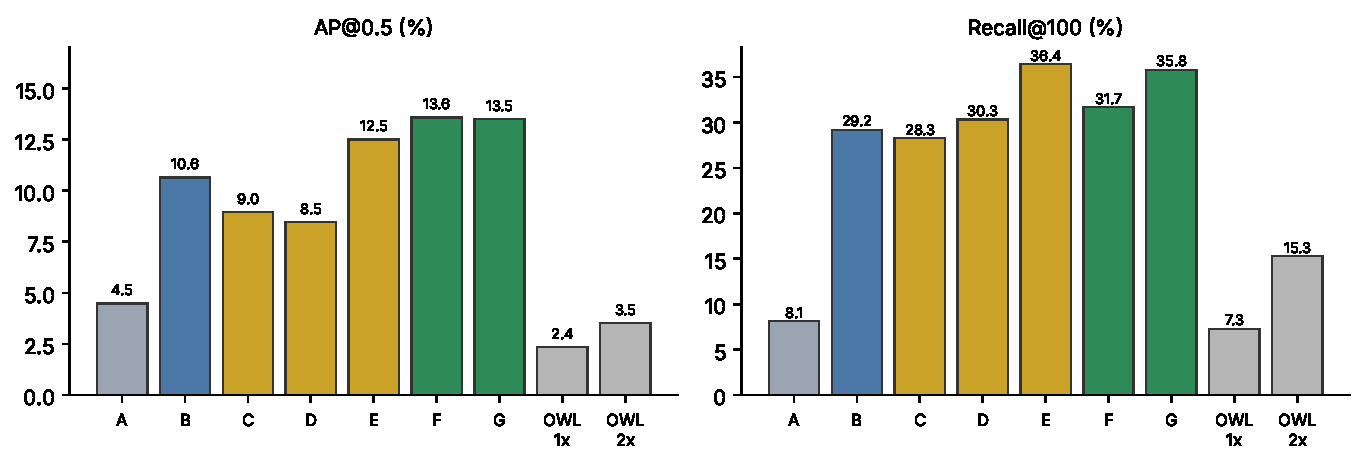
\includegraphics[width=\linewidth]{fig_ablation.pdf}
  \caption{\ap{} and Recall@100 for each configuration (data of Table~\ref{tab:main}).}
  \label{fig:ablation}
\end{figure}

\noindent\textbf{Main ablation.} Table~\ref{tab:main} and Fig.~\ref{fig:ablation} show the results, and Table~\ref{tab:ci} gives paired bootstrap 95\% confidence intervals for differences (10{,}000 resamples, episodes as units, no correction for multiple comparisons; episodes from the same image are not independent, so the intervals are indicative).

\begin{table}[t]
\centering\small
\setlength{\tabcolsep}{3pt}
\begin{tabular}{@{}lcc@{}}
\toprule
Comparison & $\Delta$\ap{} [95\% CI] & $\Delta$R@100 [95\% CI]\\
\midrule
B $-$ A (pyramid) & $+6.15$ [$+3.74,+8.59$] & --\\
C $-$ B (adaptive) & $-1.66$ [$-3.37,-0.09$] & --\\
D $-$ C (rotation) & $-0.49$ [$-1.40,+0.56$] & --\\
E $-$ D (refine) & $+4.03$ [$+2.53,+5.60$] & --\\
\midrule
F $-$ B (refine) & $+2.95$ [$+1.59,+4.36$] & $+2.52$ [$+0.58,+4.49$]\\
G $-$ F (rotation) & $-0.09$ [$-1.25,+0.96$] & $+4.12$ [$+1.78,+6.57$]\\
E $-$ B & $+1.87$ [$-0.54,+4.18$] & $+7.25$ [$+2.52,+11.98$]\\
F $-$ E & $+1.07$ [$-1.13,+3.37$] & $-4.73$ [$-9.45,-0.03$]\\
\bottomrule
\end{tabular}
\caption{Paired differences between configurations (percentage points). A dash means the interval was not computed.}
\label{tab:ci}
\end{table}

We draw four conclusions. (1) \emph{Multi-scale search matters}: the fixed pyramid improves \ap{} by 6.2 points over single-scale matching. (2) \emph{Coarse-to-fine refinement is the most useful component}: on the fixed pyramid it adds 3.0 \ap{} points and 2.5 recall points, and both intervals exclude zero. (3) \emph{Rotation helps recall but not AP}: on top of F it adds 4.1 Recall@100 points while \ap{} is unchanged ($-0.09$, interval spanning zero). (4) \emph{The query-adaptive pyramid did not help}: it was 1.7 points \emph{below} the fixed pyramid, with an interval that only barely excludes zero, so we read it as weak evidence of harm, not as proof. We did not test why; a plausible but unverified explanation is that the size of a query taken from a different image is a noisy estimate of the target object's size.

The full adaptive pipeline E is not significantly different from the plain fixed pyramid B on AP (interval spans zero), although it has much higher recall (+7.25). G has AP and recall comparable to E (36.4 vs.\ 35.8 Recall@100; we did not test G against E directly) while being faster (3.04 s against 3.74 s) and not depending on the adaptive pyramid, which did not help; this is why we use G as the final method.

\begin{table}[t]
\centering\small
\begin{tabular}{@{}lccc@{}}
\toprule
Method & Small & Medium & Large\\
\midrule
A Single scale & 1.93 & 8.14 & 8.23\\
B Fixed pyramid & 8.60 & 13.63 & 13.35\\
C Adaptive & 8.17 & 9.50 & 12.24\\
D C + rotation & 7.62 & 9.60 & 10.18\\
E D + refine & 12.67 & 11.03 & 16.53\\
F B + refine & 12.06 & 15.91 & 15.33\\
G F + rotation & 12.13 & 14.93 & \textbf{17.20}\\
\midrule
OWL-ViT $1\times$ & 0.10 & 2.44 & 16.25\\
OWL-ViT $2\times$ & 2.09 & 3.91 & 11.33\\
\bottomrule
\end{tabular}
\caption{\ap{} (\%) by object size. Small $<32$ px, medium 32--64 px, large $>64$ px (median longer box side). We did not compute confidence intervals per bucket.}
\label{tab:size}
\end{table}

\noindent\textbf{Comparison with OWL-ViT.} Tiled OWL-ViT scores 2.4 and 3.5 \ap{} overall. It is competitive only on large objects (16.3 against 17.2 for G, no interval computed) and almost fails on small ones (0.1--2.1 against 12.1), which dominate aerial imagery (Table~\ref{tab:size}). We caution that the baseline was not tuned and that low-resolution crops of tiny queries may disadvantage it; the result shows that off-the-shelf tiled OWL-ViT is a weak baseline in this setting, not that image-guided detection is inherently weak.

\noindent\textbf{Localisation is the main bottleneck.} Table~\ref{tab:iou} shows the AP of G at three IoU thresholds. AP nearly triples when the threshold is relaxed from 0.5 to 0.1, which means many detections fall on or near a correct object but with a box that is not tight enough. Our output box size is the query box size rescaled by the pyramid level, so it is wrong whenever the query object and the target object differ in size. The value at IoU 0.1 is an upper-bound indication only, since in crowded scenes a loose box can match a neighbouring instance. Even at IoU 0.1 AP is 37.8, so detection itself is also limited.

\begin{table}[t]
\centering\small
\begin{tabular}{@{}lccc@{}}
\toprule
IoU threshold & 0.1 & 0.3 & 0.5\\
\midrule
AP of G (\%) & 37.75 & 26.22 & 13.50\\
\bottomrule
\end{tabular}
\caption{Average precision of the final method G at different IoU thresholds (117 episodes).}
\label{tab:iou}
\end{table}

\subsection{Qualitative results}
Figure~\ref{fig:qual} shows the highest- and lowest-AP episodes for G. The method works best in dense scenes with objects of the same type and similar scale to the query (for example, cars in a traffic jam). Failure modes visible in our qualitative examples include: (i) \emph{box size mismatch}, where the query object is much larger or smaller than the target objects, so detections are on the right region with wrong box size; (ii) \emph{appearance gap}, with dark, blurred, or overexposed queries or targets; (iii) \emph{class confusion}, where e.g.\ a truck query returns cars and vans; and (iv) \emph{duplicates}, since NMS at IoU 0.5 does not merge nested boxes of different sizes on one object. The figures show the top 40 detections regardless of score, which makes them look more cluttered than the ranking suggests.

\begin{figure*}[t]
  \centering
  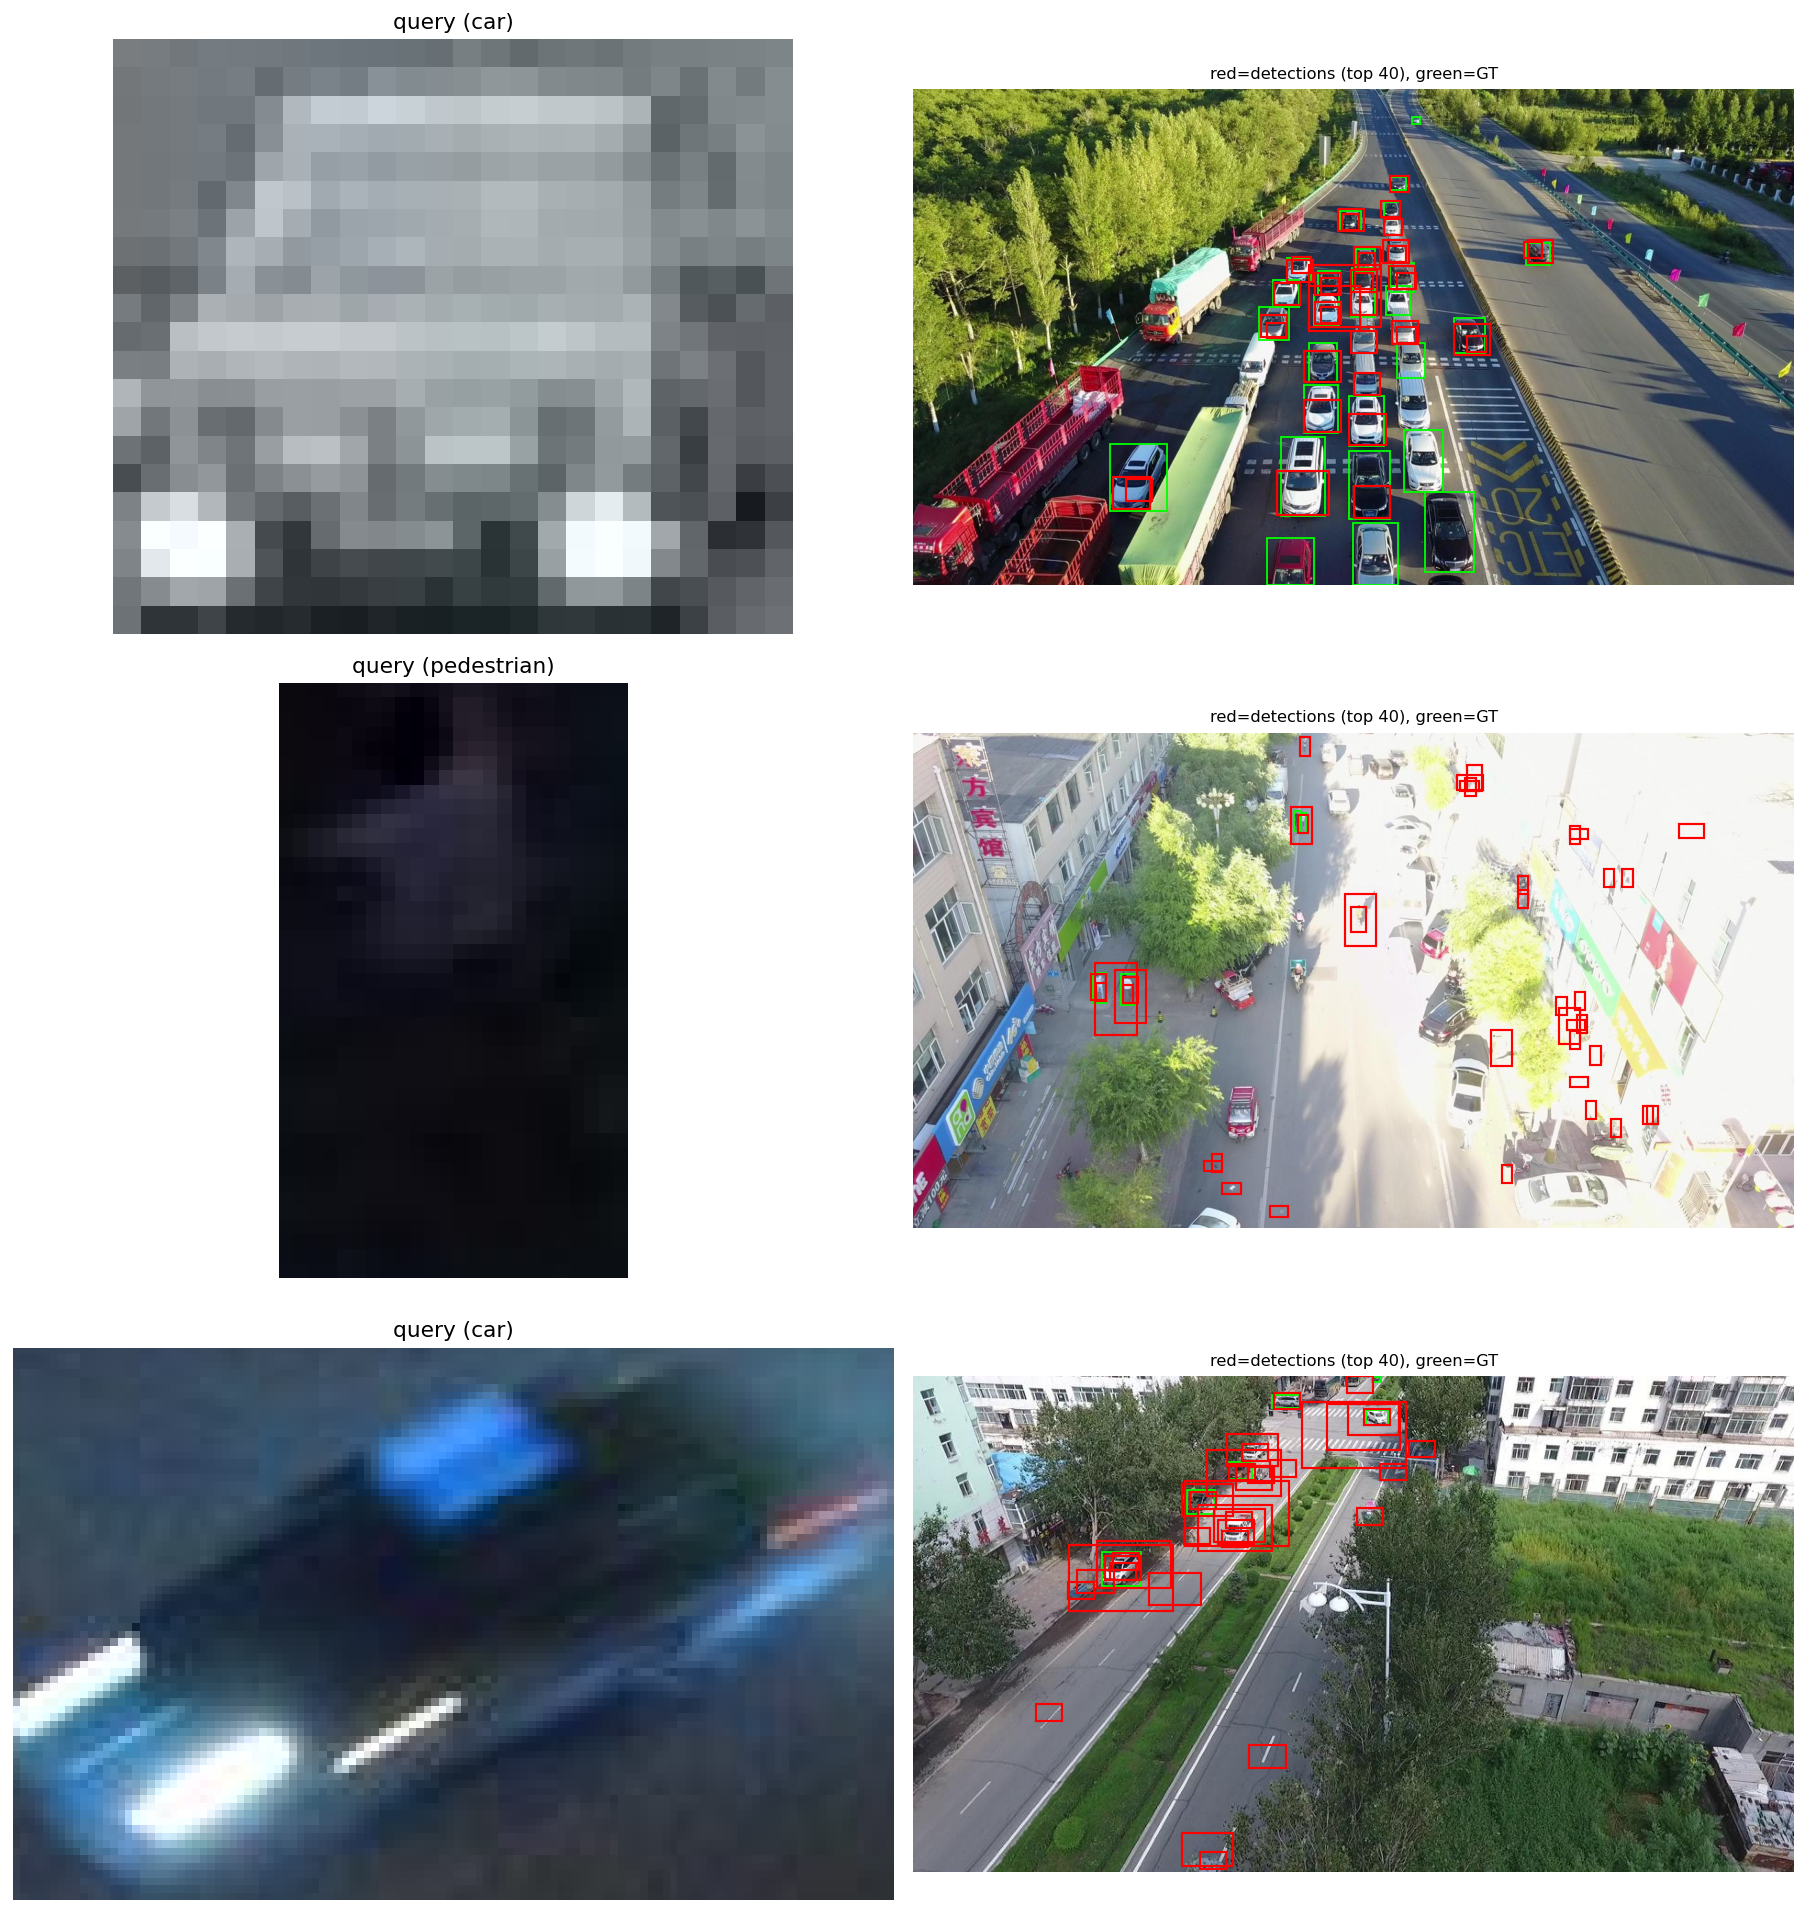
\includegraphics[width=0.49\linewidth]{qual_success.png}\hfill
  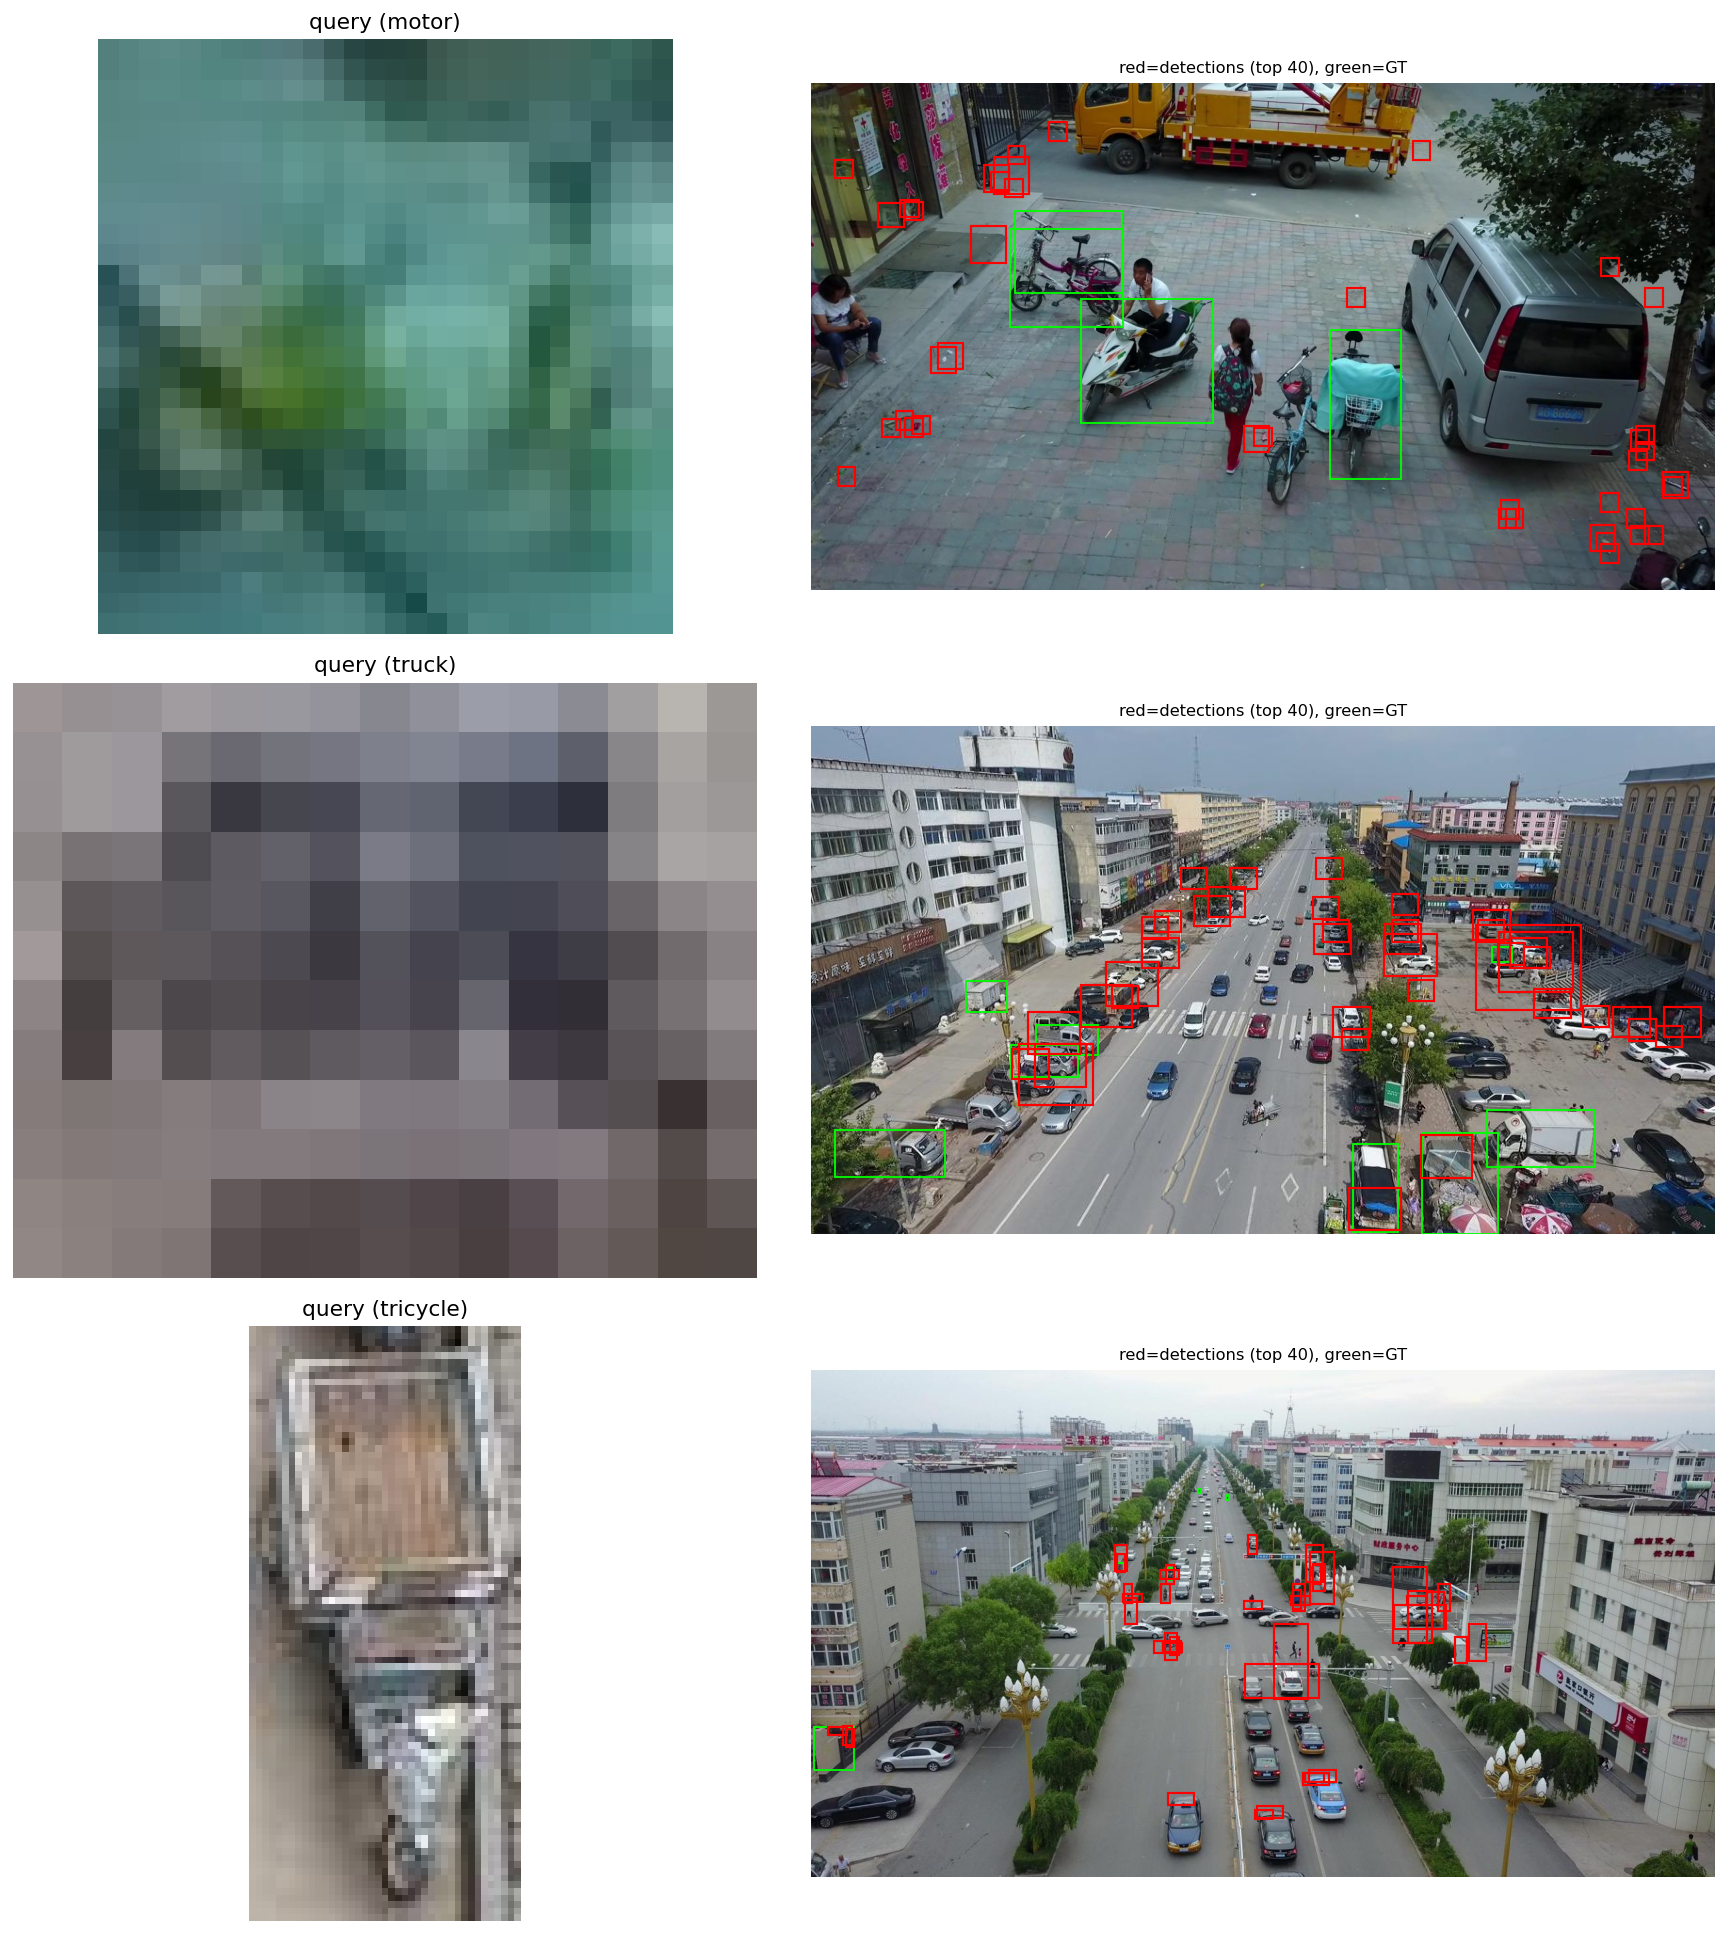
\includegraphics[width=0.49\linewidth]{qual_failure.png}
  \caption{Left: highest-AP episodes of G. Right: lowest-AP episodes of G. In each row, the left panel is the query crop (enlarged for display; the model actually receives the surrounding context window, rescaled so the object spans $n_p$ patches) and the right panel shows the top-40 detections (red) and ground truth (green). These are best and worst cases, not typical ones.}
  \label{fig:qual}
\end{figure*}

%------------------------------------------------------------------------
\section{Interactive Demo}
\label{sec:demo}
We provide a Gradio demo (Fig.~\ref{fig:demo}) built on the same code as the experiments (final configuration G). The user uploads a drone image, clicks two opposite corners of an object, and receives the matching boxes with their scores and matched rotation; settings allow switching rotation and refinement on or off and changing the score threshold. The first search on a new image builds the feature pyramid (a few seconds), and later queries on the same image reuse it. Two caveats apply. First, the demo marks the query on the \emph{same} image, which is an easier setting than the cross-image queries of our experiments and was not evaluated. Second, the demo can merge overlapping boxes for display (on by default, switchable); this clean-up is not part of the evaluated pipeline, and no number in this report uses it. Fig.~\ref{fig:demo} is a single illustrative example, not a result. The demo code is listed in Appendix~\ref{app:code}.

\begin{figure}[t]
  \centering
  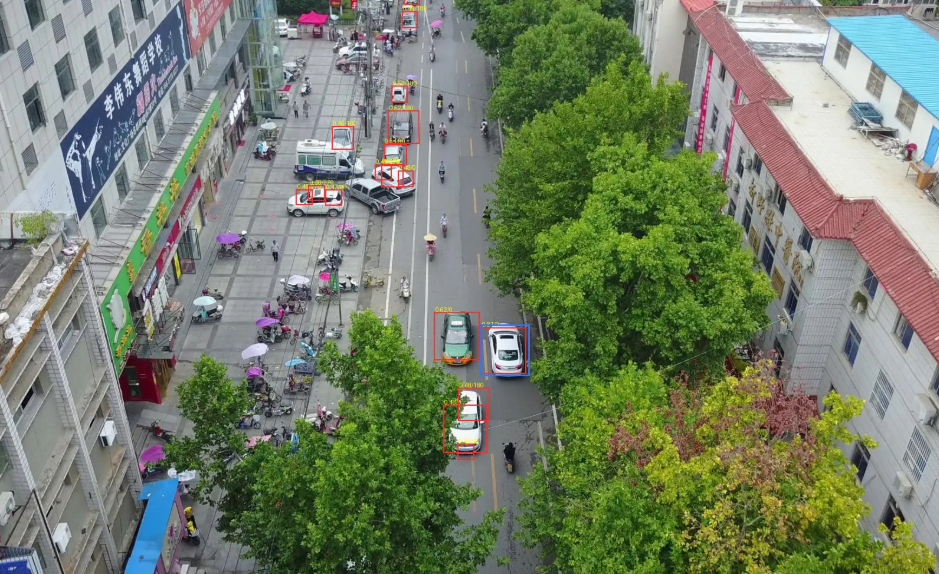
\includegraphics[width=\linewidth]{fig_demo.png}
  \caption{Demo output for a query on the white car (blue box). Red boxes show matches with score and matched rotation. One example selected by hand, not a measured result.}
  \label{fig:demo}
\end{figure}

%------------------------------------------------------------------------
\section{Limitations and Discussion}
\label{sec:limits}

\begin{itemize}
  \item \textbf{Small evaluation.} 117 episodes on 60 images, one seed, one dataset. Several intervals are wide, and some conclusions (adaptive pyramid, E vs.\ B on AP) are not firm.
  \item \textbf{Post-hoc selection.} G was selected after seeing results on the same episodes; $n_p$ was tuned on held-out images but with few episodes.
  \item \textbf{Box size is inherited from the query.} This is the largest identified weakness (Table~\ref{tab:iou}). Predicting the box extent from the matched patches is a natural next step but is untested.
  \item \textbf{Cross-image queries.} Query quality varies (blur, darkness, tiny crops), and the scale between support and target differs. The behaviour with same-image queries, as in an interactive demo, was not evaluated.
  \item \textbf{No supervised reference.} We did not train a closed-set detector for comparison; it would likely score higher on the ten VisDrone classes but cannot search for new objects.
  \item \textbf{Cost.} About 3 s per episode on a GPU for the final method. Orientation is output but not evaluated.
\end{itemize}

%------------------------------------------------------------------------
\section{Conclusion}
\label{sec:conclusion}
We built and evaluated a training-free system for query-by-example object search in drone images using DINOv2 patch matching, tiling, rotation-aware query encoding, and coarse-to-fine refinement. In our experiments, refinement is the component that reliably helps, rotation improves recall, and an adaptive scale pyramid does not help. The main open problem is box localisation. The code and all numbers in this report are reproducible from the appendix and the repository below.

%------------------------------------------------------------------------
\section*{Individual Contribution}
This project was carried out individually by Ashish Pratap Singh. I designed the pipeline and experiments, ran all experiments on Kaggle, analysed the results, and wrote this report and the code. I used an AI assistant (Claude, Anthropic) to help draft the report text; I ran all experiments and checked all reported numbers myself.

\section*{Links}
\begingroup\raggedright\sloppy
\noindent Code repository (experiments and demo): \url{https://github.com/aash-singh/EE604-Course-Project-Object-Detection-in-Drone-Images}\\
VisDrone dataset: \url{https://github.com/VisDrone/VisDrone-Dataset}\\
DINOv2 code: \url{https://github.com/facebookresearch/dinov2}; weights: \url{https://huggingface.co/facebook/dinov2-base}\\
OWL-ViT weights: \url{https://huggingface.co/google/owlvit-base-patch32}
\endgroup

{\small
\bibliographystyle{ieeetr}
\bibliography{main}
}

%------------------------------------------------------------------------
\clearpage
\appendix
\section{Hyper-parameter tuning on held-out images}
\label{app:tuning}
Tuning episodes come from VisDrone val images disjoint from the 60 evaluation images (seed 1). ``Fixed'' and ``adaptive'' use one rotation and no refinement; ``full'' is the adaptive pyramid with 4 rotations and refinement (configuration E).

\begin{table}[h]
\centering\small
\begin{tabular}{@{}lccc@{}}
\toprule
Setting & \ap{} & R@100 & s/ep\\
\midrule
fixed, $n_p{=}3$ & 6.64 & 26.87 & 1.19\\
adaptive, $n_p{=}3$ & 6.55 & 25.63 & 1.58\\
full, $n_p{=}3$ & 12.34 & 34.98 & 2.93\\
fixed, $n_p{=}4$ & 7.90 & 26.23 & 1.19\\
adaptive, $n_p{=}4$ & 8.48 & 27.98 & 1.90\\
full, $n_p{=}4$ & 10.30 & 34.64 & 3.90\\
fixed, $n_p{=}5$ & 7.79 & 21.01 & 1.19\\
adaptive, $n_p{=}5$ & 9.29 & 26.43 & 2.00\\
full, $n_p{=}5$ & 10.84 & 33.96 & 5.04\\
fixed, $n_p{=}6$ & 6.50 & 18.01 & 1.19\\
adaptive, $n_p{=}6$ & 8.62 & 25.49 & 2.04\\
full, $n_p{=}6$ & 10.41 & 30.09 & 5.91\\
\bottomrule
\end{tabular}
\caption{Tuning results (\%). We selected $n_p=4$; the full pipeline was highest at $n_p=3$ here.}
\end{table}

\section{Reproducibility}
Models: \texttt{facebook/dinov2-base} and \texttt{google/owlvit-base-patch32} from the HuggingFace hub. Random seeds: 0 for evaluation episodes, 1 for tuning episodes, 0 for the bootstrap. The OWL-ViT rows of Table~\ref{tab:main} come from the first full run, on the same 117 episodes (same seed) as our configurations.

\section{Complete code}
\label{app:code}
\subsection{Experiments (notebook code)}
The complete notebook code (all cells, in the order they were developed) follows. The same file is in the repository.

\lstinputlisting{code_appendix.py}

\subsection{Interactive demo (Gradio cell)}
\lstinputlisting{demo_code.py}

\end{document}